%% start of file `cv_german.tex', based on `template_en.tex` by Xavier Danaux (xdanaux@gmail.com).
% This work may be distributed and/or modified under the
% conditions of the LaTeX Project Public License version 1.3c,
% available at http://www.latex-project.org/lppl/.
% 
% Thomas Quaritsch <t.quaritsch@student.tugraz.at>

\documentclass[11pt,a4paper]{moderncv}

\usepackage[german]{babel}
\usepackage{moderncv-additions}
\usepackage{pdfpages}

% moderncv themes
\moderncvtheme{casual}   % optional arguments are 'blue' (default), 'orange', 'red', 'green', 'grey' and 'roman' (for roman fonts, instead of sans serif fonts)
%\moderncvtheme[green]{classic}                % idem

% character encoding
\usepackage[utf8]{inputenc}                   % replace by the encoding you are using

% adjust the page margins
\usepackage[scale=0.8]{geometry}
\setlength{\hintscolumnwidth}{3cm}			  % if you want to change the width of the column with the dates
%\AtBeginDocument{\setlength{\maketitlenamewidth}{6cm}}  % only for the classic theme, if you want to change the width of your name placeholder (to leave more space for your address details


\AtBeginDocument{\recomputelengths}           % required when changes are made to page layout lengths

% personal data
\firstname{Simon}
\familyname{Szustkowski}
%\title{Resumé title (optional)}               % optional, remove the line if not wanted
\address{Marsbruchstraße 117}{44287 Dortmund}        % optional, remove the line if not wanted
\mobile{+49 231 3306614}                     % optional, remove the line if not wanted
%\phone{phone (optional)}                      % optional, remove the line if not wanted
%\fax{fax (optional)}                          % optional, remove the line if not wanted
\email{mail@simonszu.de}                      % optional, remove the line if not wanted
%\extrainfo{additional information (optional)} % optional, remove the line if not wanted
\photo[64pt]{picture}                          % '64pt' is the height the picture must be resized to and 'picture' is the name of the picture file; optional, remove the line if not wanted
%\quote{``Das ist ein toller Frusterspruch\\ von Friede Frusterfrau.'' -- Friede Frusterfrau}                 % optional, remove the line if not wanted

%\nopagenumbers{}                             % uncomment to suppress automatic page numbering for CVs longer than one page


%----------------------------------------------------------------------------------
%            content
%----------------------------------------------------------------------------------

\begin{document}

% color redefinitions must be after \begin{document}!
\definecolor{firstnamecolor}{RGB}{125,85,85}
\definecolor{familynamecolor}{RGB}{138,74,57}
\definecolor{quotecolor}{RGB}{125,85,85}
\definecolor{addresscolor}{RGB}{125,85,85}
\definecolor{sectionrectanglecolor}{RGB}{138,74,57}
\definecolor{sectiontitlecolor}{RGB}{138,74,57}
\definecolor{subsectioncolor}{RGB}{125,85,85}
\definecolor{footersymbolcolor}{RGB}{125,85,85}	

\makeatletter

\pagestyle{empty}
\chapter*{Bewerbungs}{unterlagen}

\vspace*{50mm}
\begin{minipage}{\textwidth}
	\vspace*{3mm}
	\familynamestyle{\@firstname}~~\firstnamestyle{\@familyname} 	
	\hspace*{5mm}{{\color{firstnamecolor}\includegraphics[width=64pt]{picture}}}\\[3mm]
	\@addressstreet, \@addresscity ~~~ \mobilesymbol~\@mobile ~~~ \emailsymbol~\@email
\end{minipage}
\begin{minipage}{70pt}
	
\end{minipage}

\vfill

\begin{minipage}{1.0\textwidth}
	\section{Inhalt}
	\tableofcontents
\end{minipage}

\newpage
\pagestyle{fancy}
%\chapter{Curriculum}{~Vit\ae}
\chapter{Lebenslauf}{}
\makequote

\section{Persönliche Daten}
%%%%%%%%%%%%%%%%%%%%%%%%%%%%%%%%%%%%%%%%%%%%%%%%%%%%%%%%%%%%%%%%%%%%
\cvline{Name}{\@firstname~\@familyname}
\cvline{Anschrift}{\@addressstreet, \@addresscity}
\cvline{Telefon}{\@mobile}
\cvline{E-Mail}{\@email}
\cvline{Geburtsdatum}{11. Februar 1988 in Münster}
\cvline{Staatsbürgerschaft}{Deutschland / Schweiz}
%\cvline{Familienstand}{ledig}
%\cvline{Präsenzdienst}{abgeleistet}
%\cvline{Führerschein}{A,B,C,D,E,F,G}
\makeatother 

%\cventry{year--year}{Degree}{Institution}{City}{\textit{Grade}}{Description}  % arguments 3 to 6 are optional

\section{Ausbildung} 
%%%%%%%%%%%%%%%%%%%%%%%%%%%%%%%%%%%%%%%%%%%%%%%%%%%%%%%%%%%%%%%%%%%%

\cventry{10/2009 -- 04/2018}{Bachelor of Science}{Technische Universität}{Dortmund}{\textit{Informatik}}{Nebenfach: Maschinenbau}  % arguments 3 to 6 are optional

\cventry{09/2006 -- 06/2009}{Mechatroniker (IHK)}{Miele \& Cie. KG}{Bielefeld}{}{Zusätzlich: Elektrofachkraft} 

\section{Berufserfahrung} 
%%%%%%%%%%%%%%%%%%%%%%%%%%%%%%%%%%%%%%%%%%%%%%%%%%%%%%%%%%%%%%%%%%%%

\cventry{12/2012 -- heute}{Consultant für Red Hat OpenShift}{Viada GmbH \& Co KG}{Dortmund}{}{}
\cventry{12/2012 -- 04/2018}{Administrator des Wide Area Networks}{ECOFIS GmbH}{Dortmund}{}{}
\cventry{10/2010 -- 11/2012}{First Level Support}{Sozialforschungsstelle der Technischen Universität}{Dortmund}{}{}
\cventry{09/2006 -- 06/2009}{Auszubildender zum Mechatroniker (IHK)}{Miele \& Cie. KG}{Bielefeld}{}{}

\section{Sprachen} 
%%%%%%%%%%%%%%%%%%%%%%%%%%%%%%%%%%%%%%%%%%%%%%%%%%%%%%%%%%%%%%%%%%%%

\cvline{Deutsch}{Muttersprache}{}
\cvline{Englisch}{fließend in Wort und Schrift}
\cvline{Französisch}{Grundkenntnisse}

\section{IT-Kompetenzen} 
%%%%%%%%%%%%%%%%%%%%%%%%%%%%%%%%%%%%%%%%%%%%%%%%%%%%%%%%%%%%%%%%%%%%

\cvline{Programmiersprachen}{Ruby, Python, Java, JavaScript, C++, Go}
\cvline{Betriebssysteme}{Red Hat Enterprise Linux, Debian Linux, Arch Linux, Apple macOS, Microsoft Windows}
\cvline{Sonstige Tools}{Red Hat OpenShift, Kubernetes, git, svn, ansible, Docker, Tensorflow, JetBrains IDE, Eclipse, LaTeX, Microsoft Office}
\newpage

\section{Auszeichnungen} 
%%%%%%%%%%%%%%%%%%%%%%%%%%%%%%%%%%%%%%%%%%%%%%%%%%%%%%%%%%%%%%%%%%%%
\cvline{01/2019}{Viada Subject Matter Expert in IT Automation and Management}
\cvline{01/2019}{Viada Subject Matter Expert in Hybrid Cloud Infrastructure Administration}
\cvline{01/2019}{Viada Subject Matter Expert in Hybrid Cloud Infrastructure Administration}

%\cvline{xx/xxxx}{Musterpreis}


\section{Außerberufliche Tätigkeiten} 
%%%%%%%%%%%%%%%%%%%%%%%%%%%%%%%%%%%%%%%%%%%%%%%%%%%%%%%%%%%%%%%%%%%%

\cvline{Chaostreff Dortmund e.V.}{Mithilfe auf und Besuch von Events im Umfeld des Chaos Computer Clubs} 
\cvline{Technisches Hilfswerk}{Technischer Helfer (zur Zeit inaktiv)}

\section{Interessen}
%%%%%%%%%%%%%%%%%%%%%%%%%%%%%%%%%%%%%%%%%%%%%%%%%%%%%%%%%%%%%%%%%%%%

\cvline{Amateurfunk}{Betrieb einer Funkstation im Amateurfunkdienst (Klasse E)}
\cvline{Fotografie}{Architektur- und Landschaftsfotografie}
\cvline{Making}{Elektro- und Programmierprojekte im Umfeld der Maker-Szene}

%\section{Publikationen} 
%%%%%%%%%%%%%%%%%%%%%%%%%%%%%%%%%%%%%%%%%%%%%%%%%%%%%%%%%%%%%%%%%%%%

%\subsection{Konferenzen und Workshops}

%\cvline{mm/jjjj}{Autor 1 und Autor 2. \textbf{Mustertitel: Unser tolles Paper.} In \textit{Proceedings of the First Muster Workshop 1970}, Musterstadt, Musterland, YYYY.}

% \newpage

%\subsection{Technical Reports}

%\cvline{....}{....}

%\cvline{....}{alternativ kann man auch BibTex verwenden:}

\renewcommand*{\refname}{Abschlussarbeiten}
\nocite{*}
\bibliographystyle{cv}
\bibliography{publications}       % 'publications' is the name of a BibTeX file


%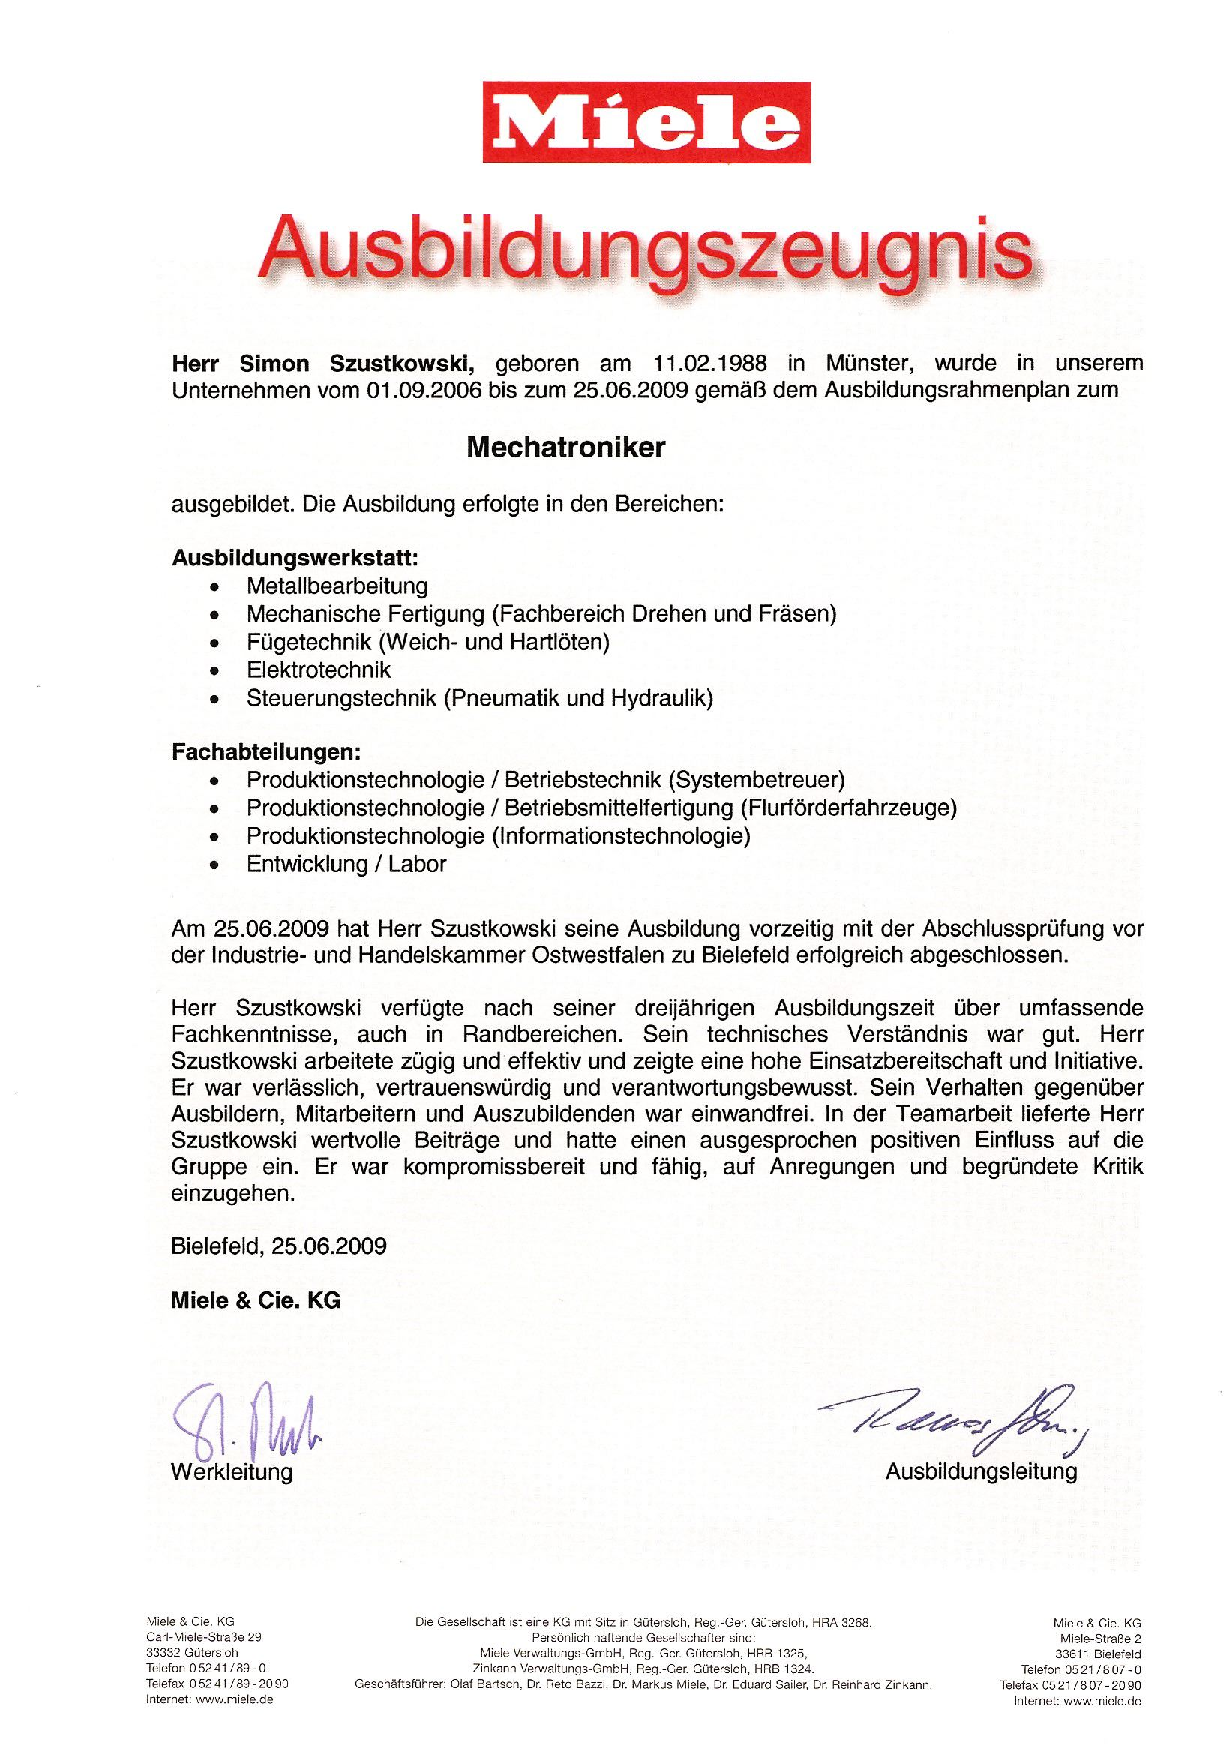
\includepdf[pages=1,addtotoc={
%	4, chapter, 1, Arbeitszeugnis Miele \& Cie. KG, az-miele
%	}]{azmiele.pdf}
\includepdf[pages=1-,addtotoc={1, section, 1, Arbeitszeugnis ECOFIS GmbH, azsfs} ]{azecofis.pdf}
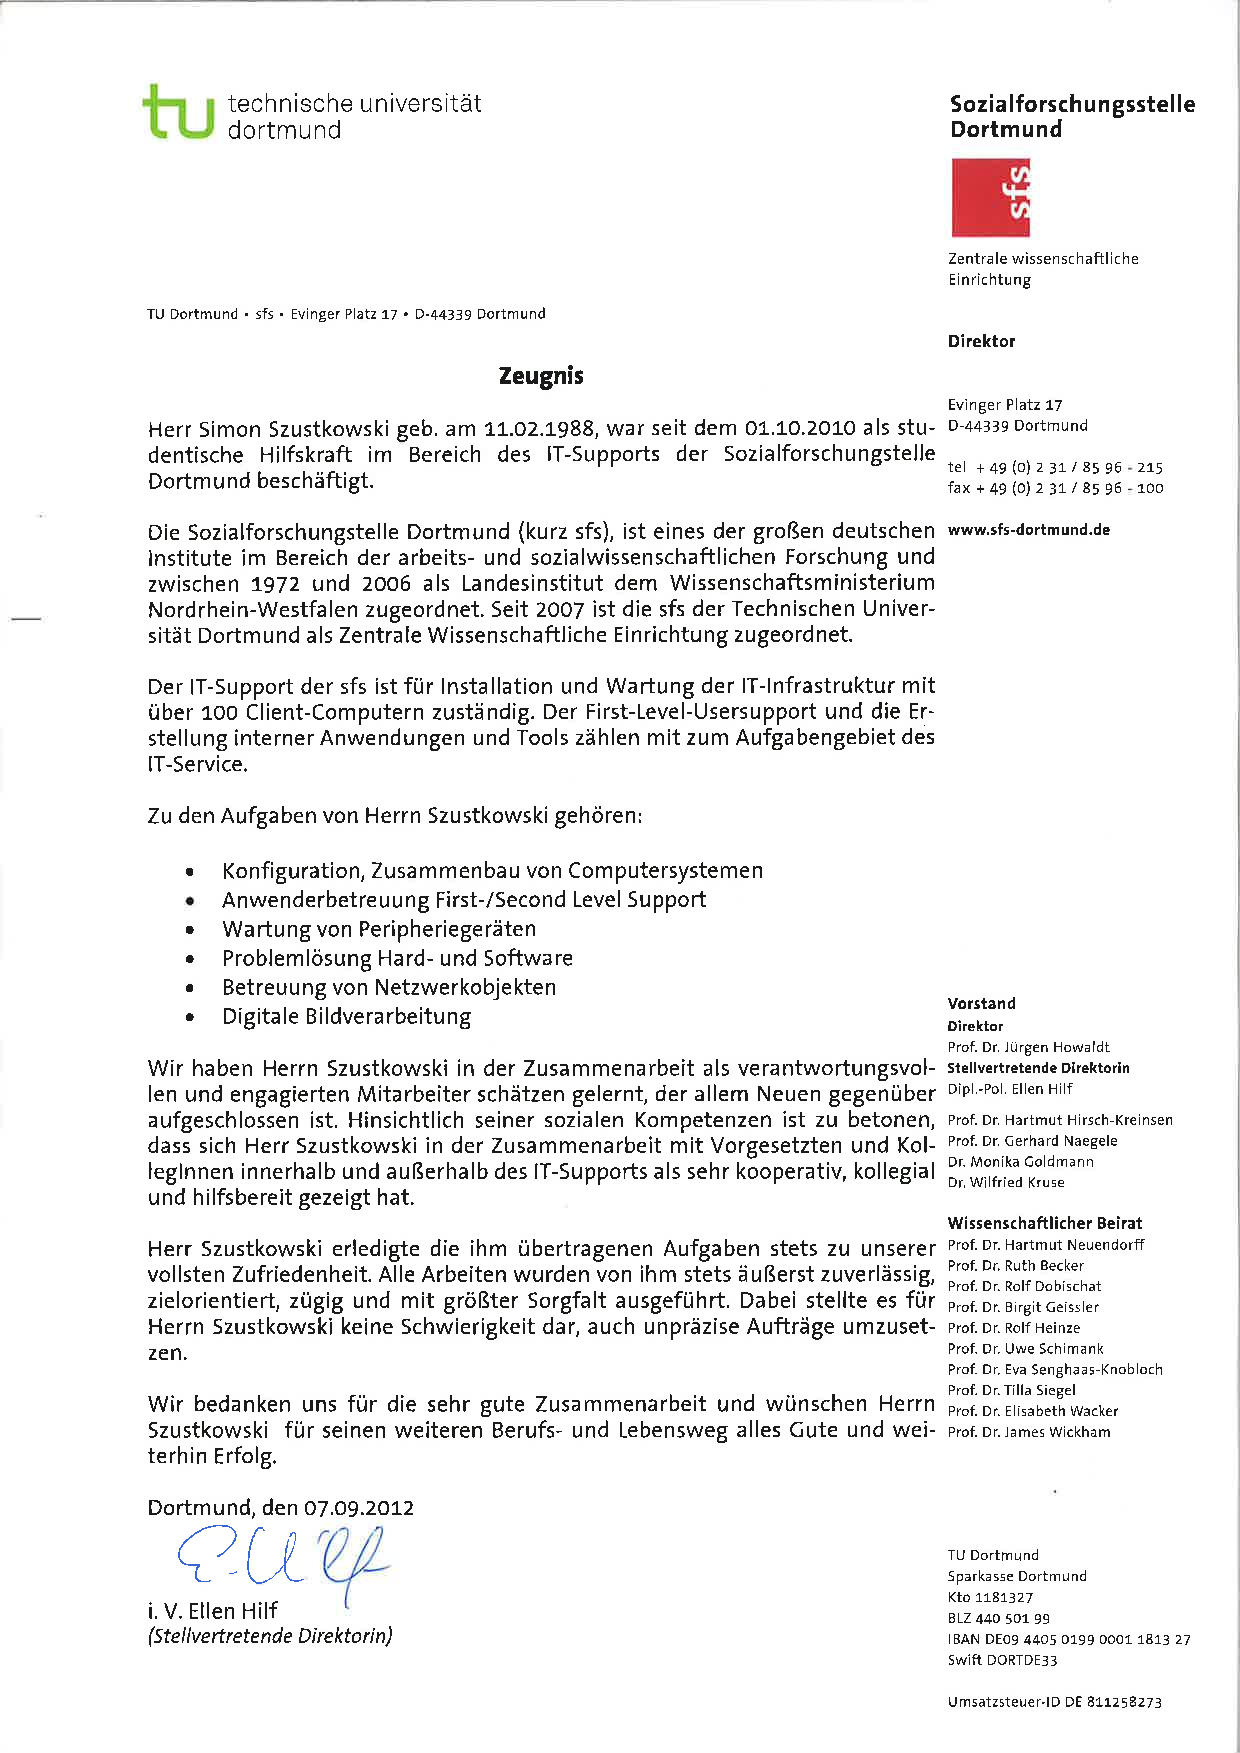
\includepdf[pages=1,addtotoc={1, section, 1, Arbeitszeugnis Sozialforschungsstelle Dortmund, azsfs} ]{azsfs.pdf}
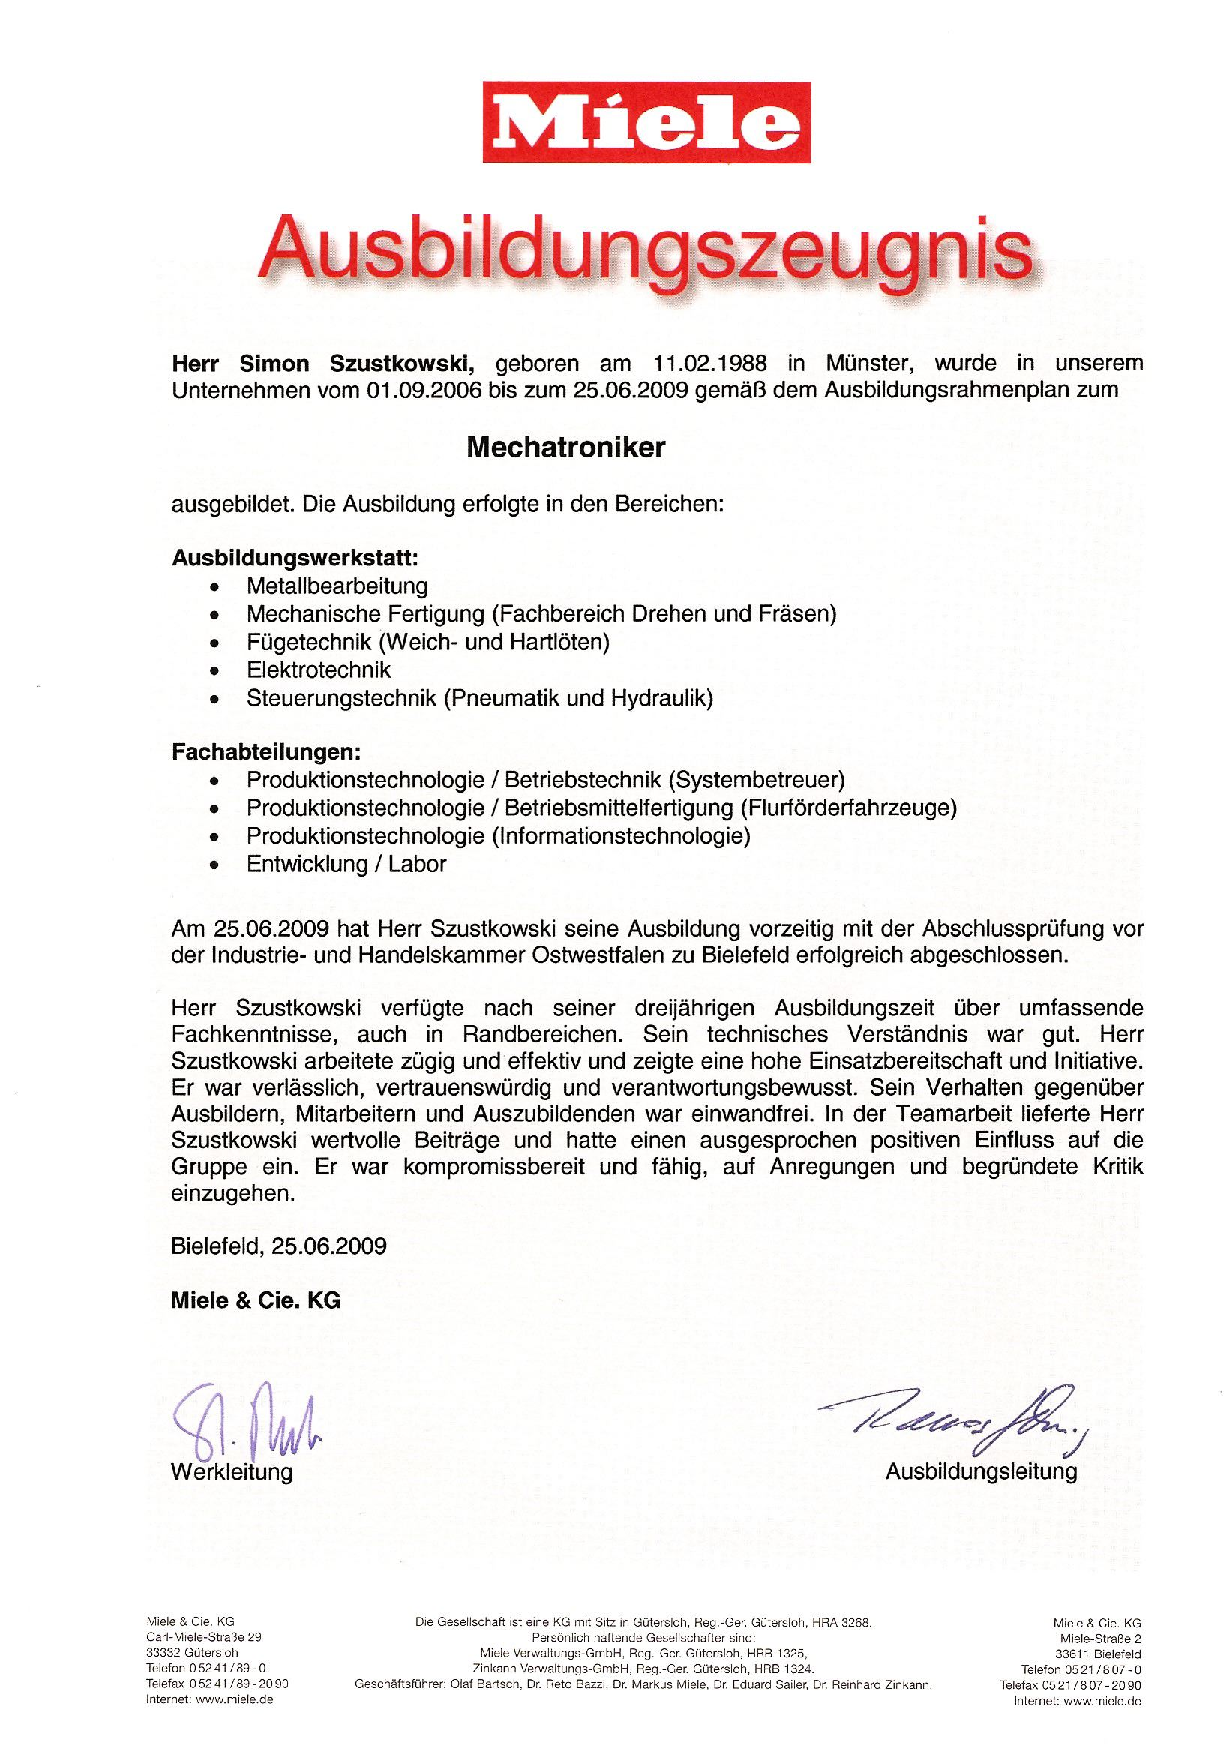
\includepdf[pages=1,addtotoc={1, section, 1, Arbeitszeugnis Miele \& Cie. KG, azmiele} ]{azmiele.pdf}
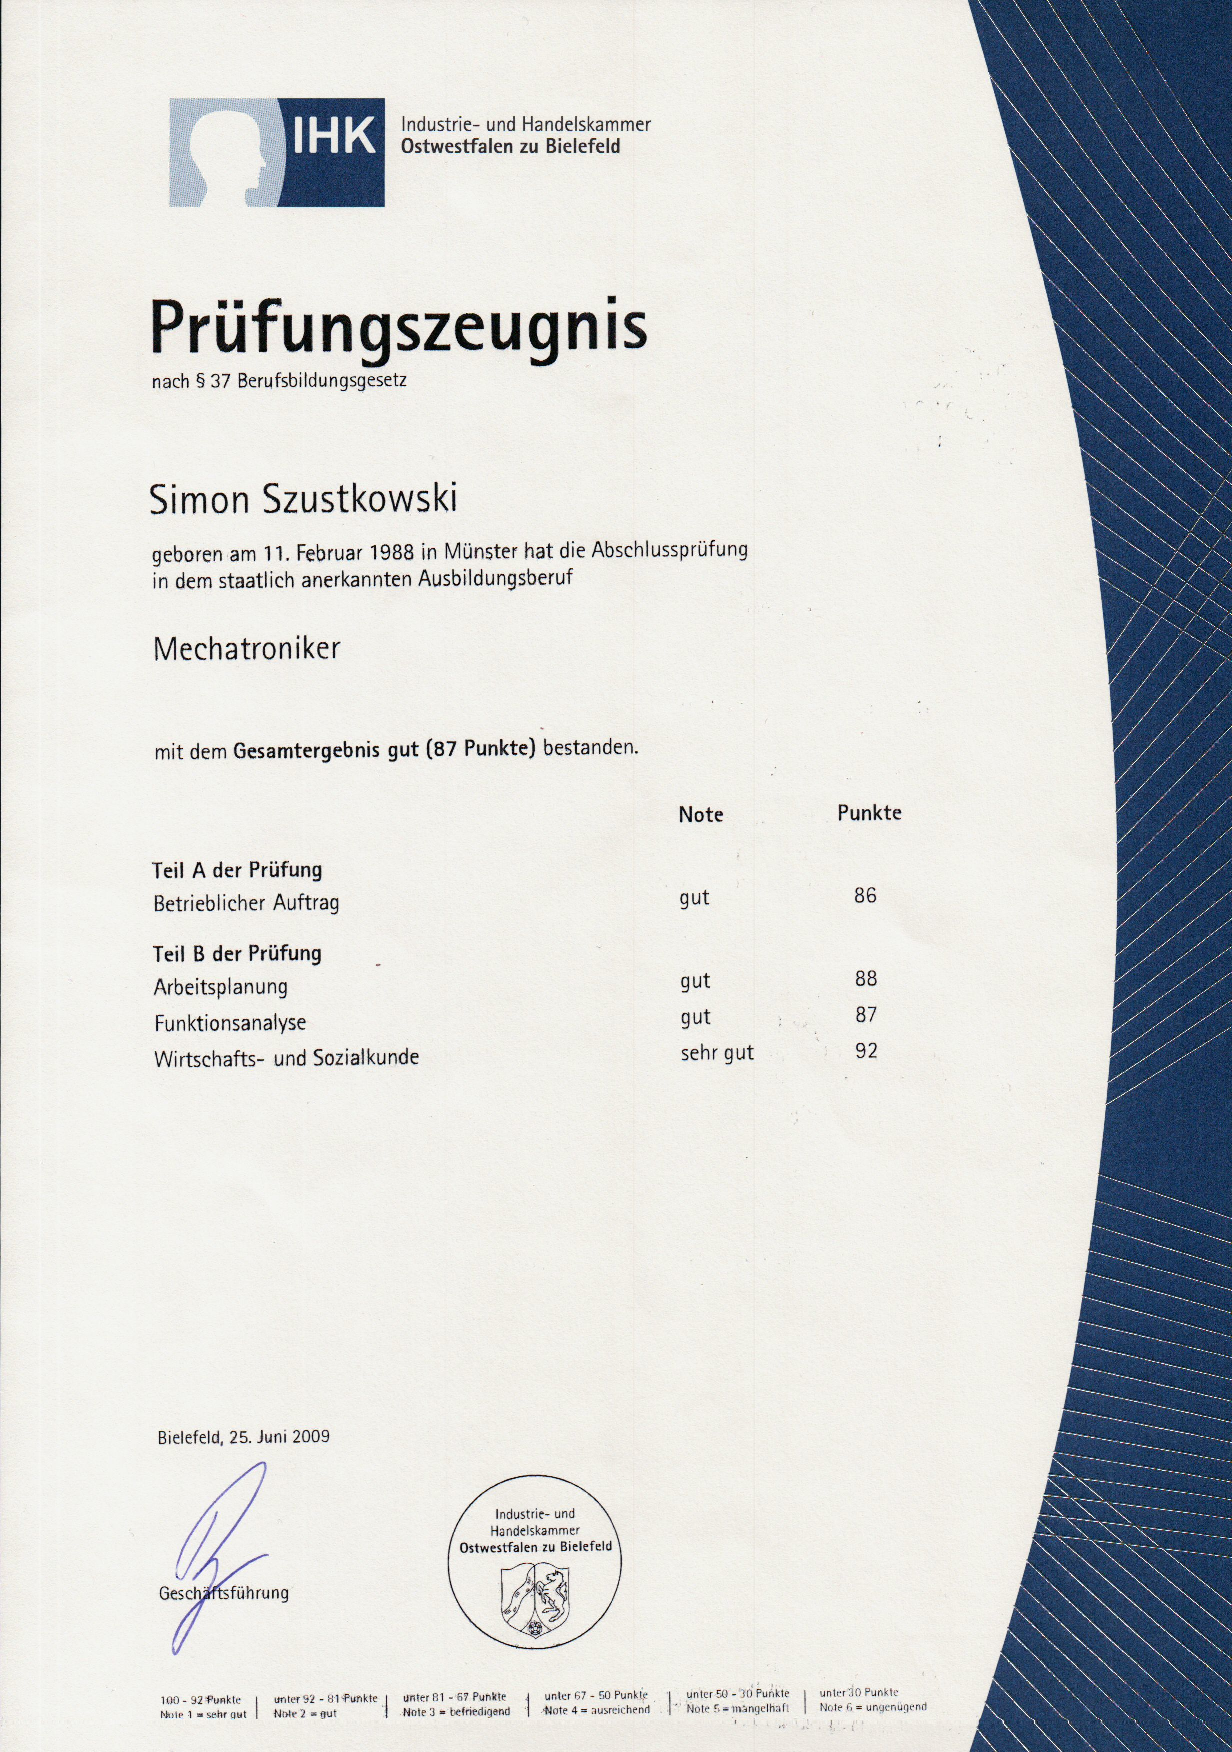
\includepdf[pages=1,addtotoc={1, section, 1, Ausbildungszeugnis, ausbildungszeugnis} ]{ausbildungszeugnis.pdf}


%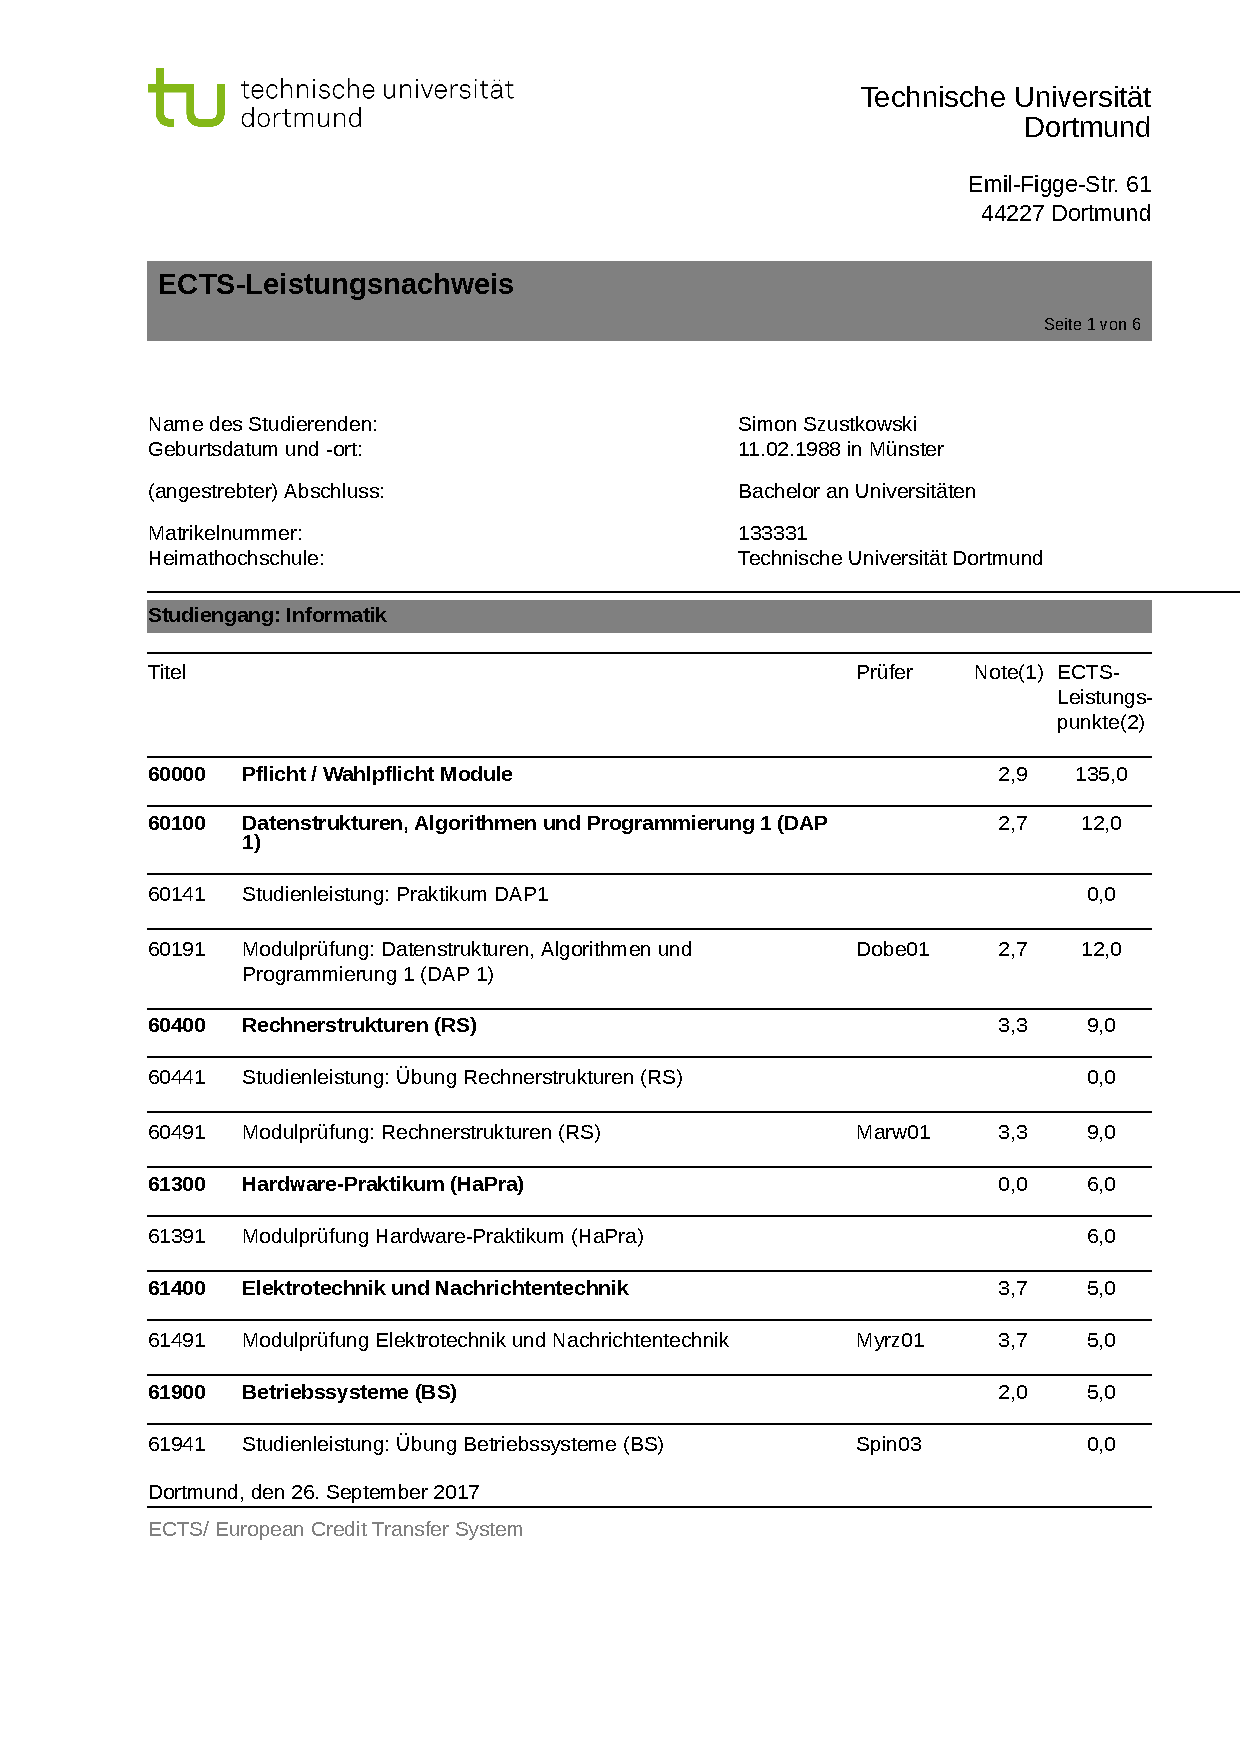
\includepdf[pages=1-,addtotoc={1, section, 1, Notenspiegel, notenspiegel} ]{notenspiegel.pdf}

%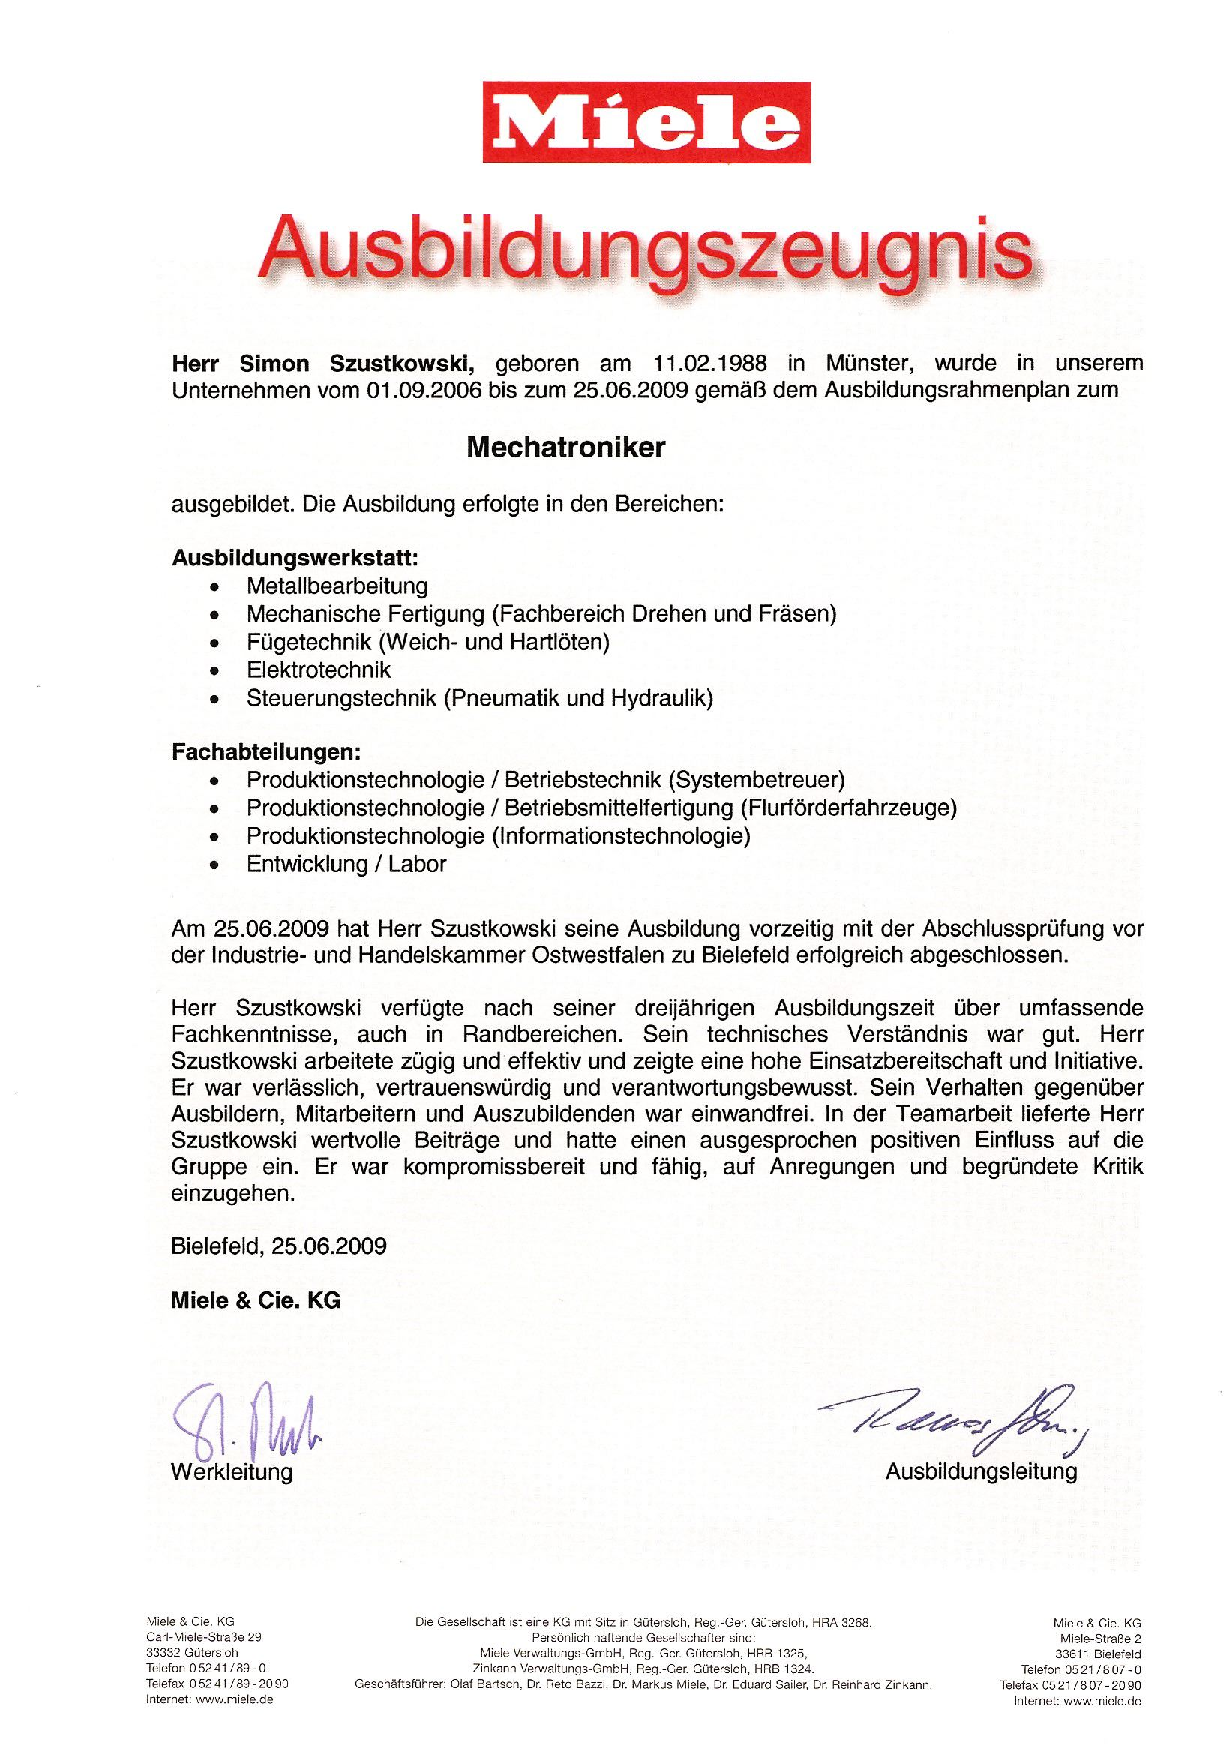
\includepdf[pages=1-,pagecommand={\chapter{Arbeitszeugnis Miele \& Cie. KG}}]{azmiele.pdf}
%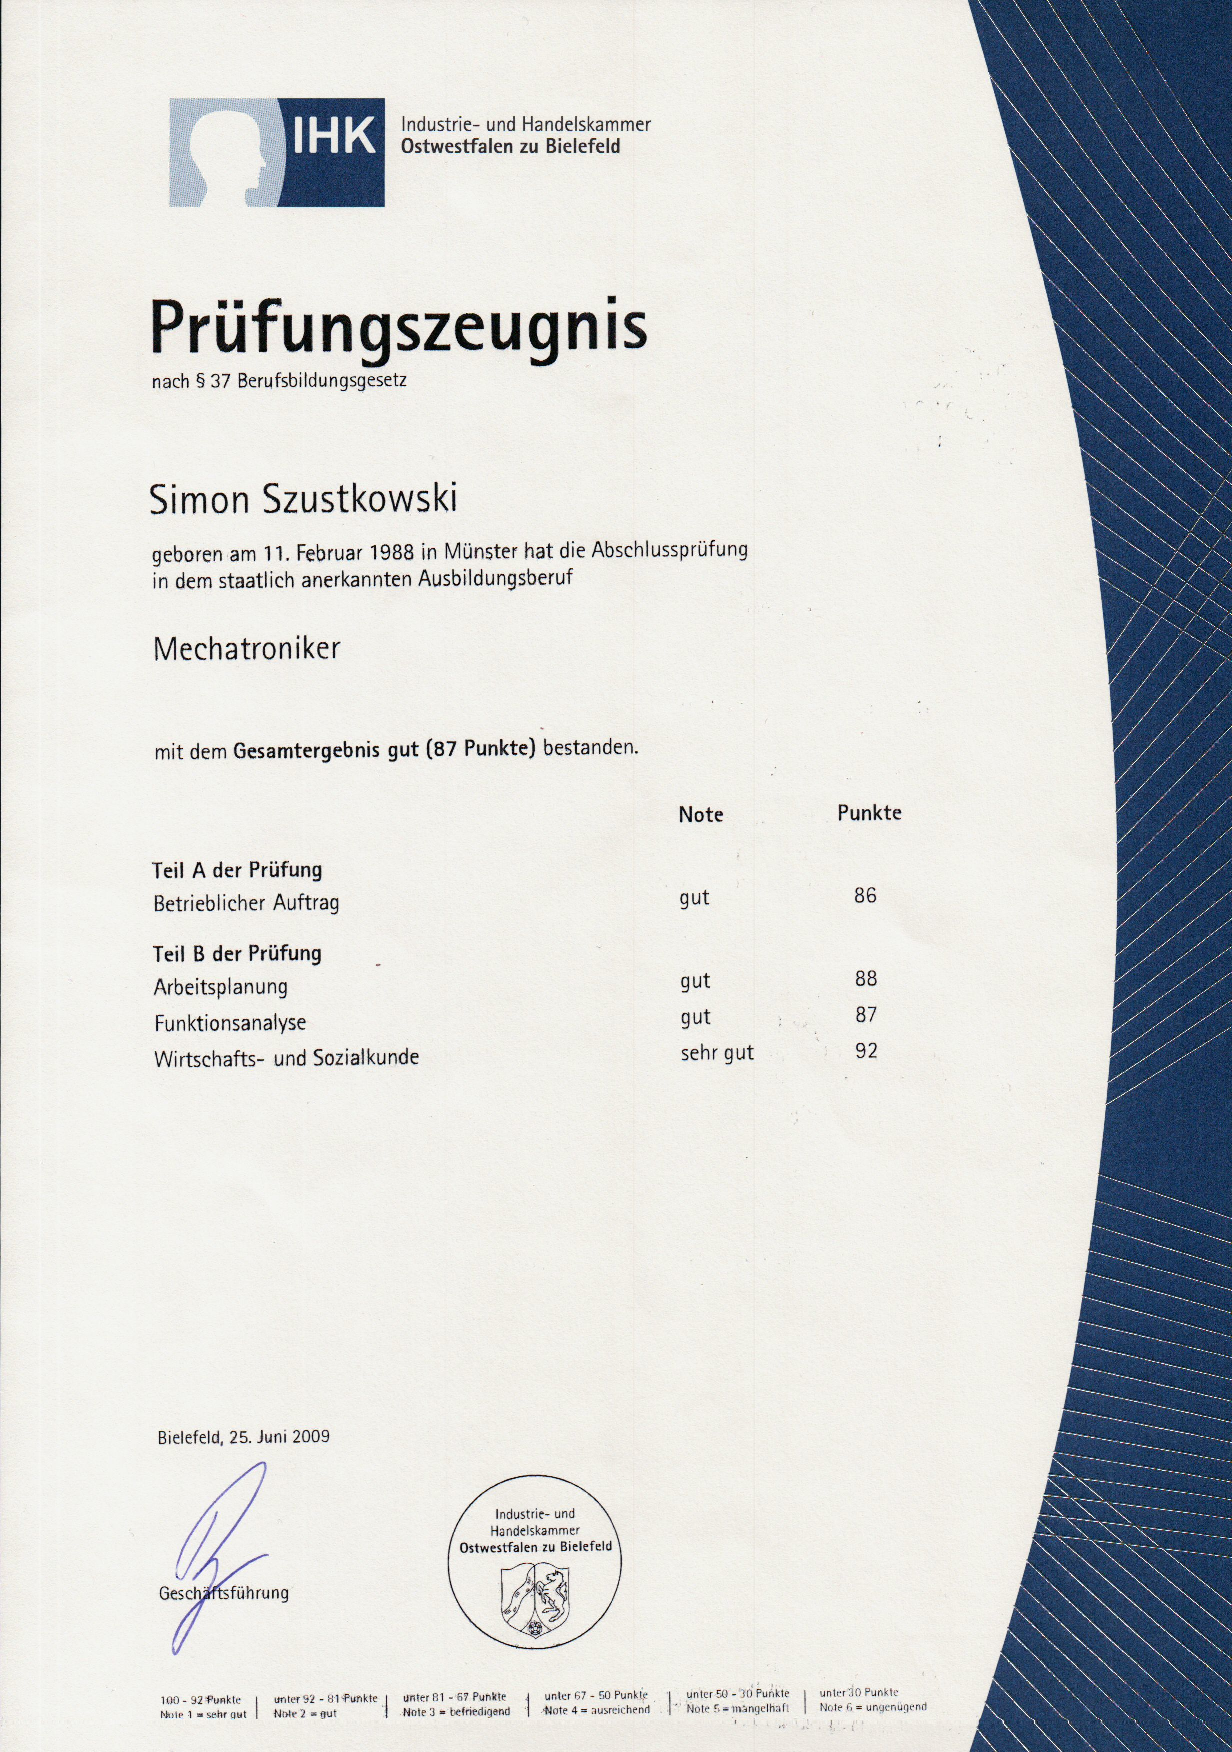
\includepdf[pages=1-]{ausbildungszeugnis.pdf}
%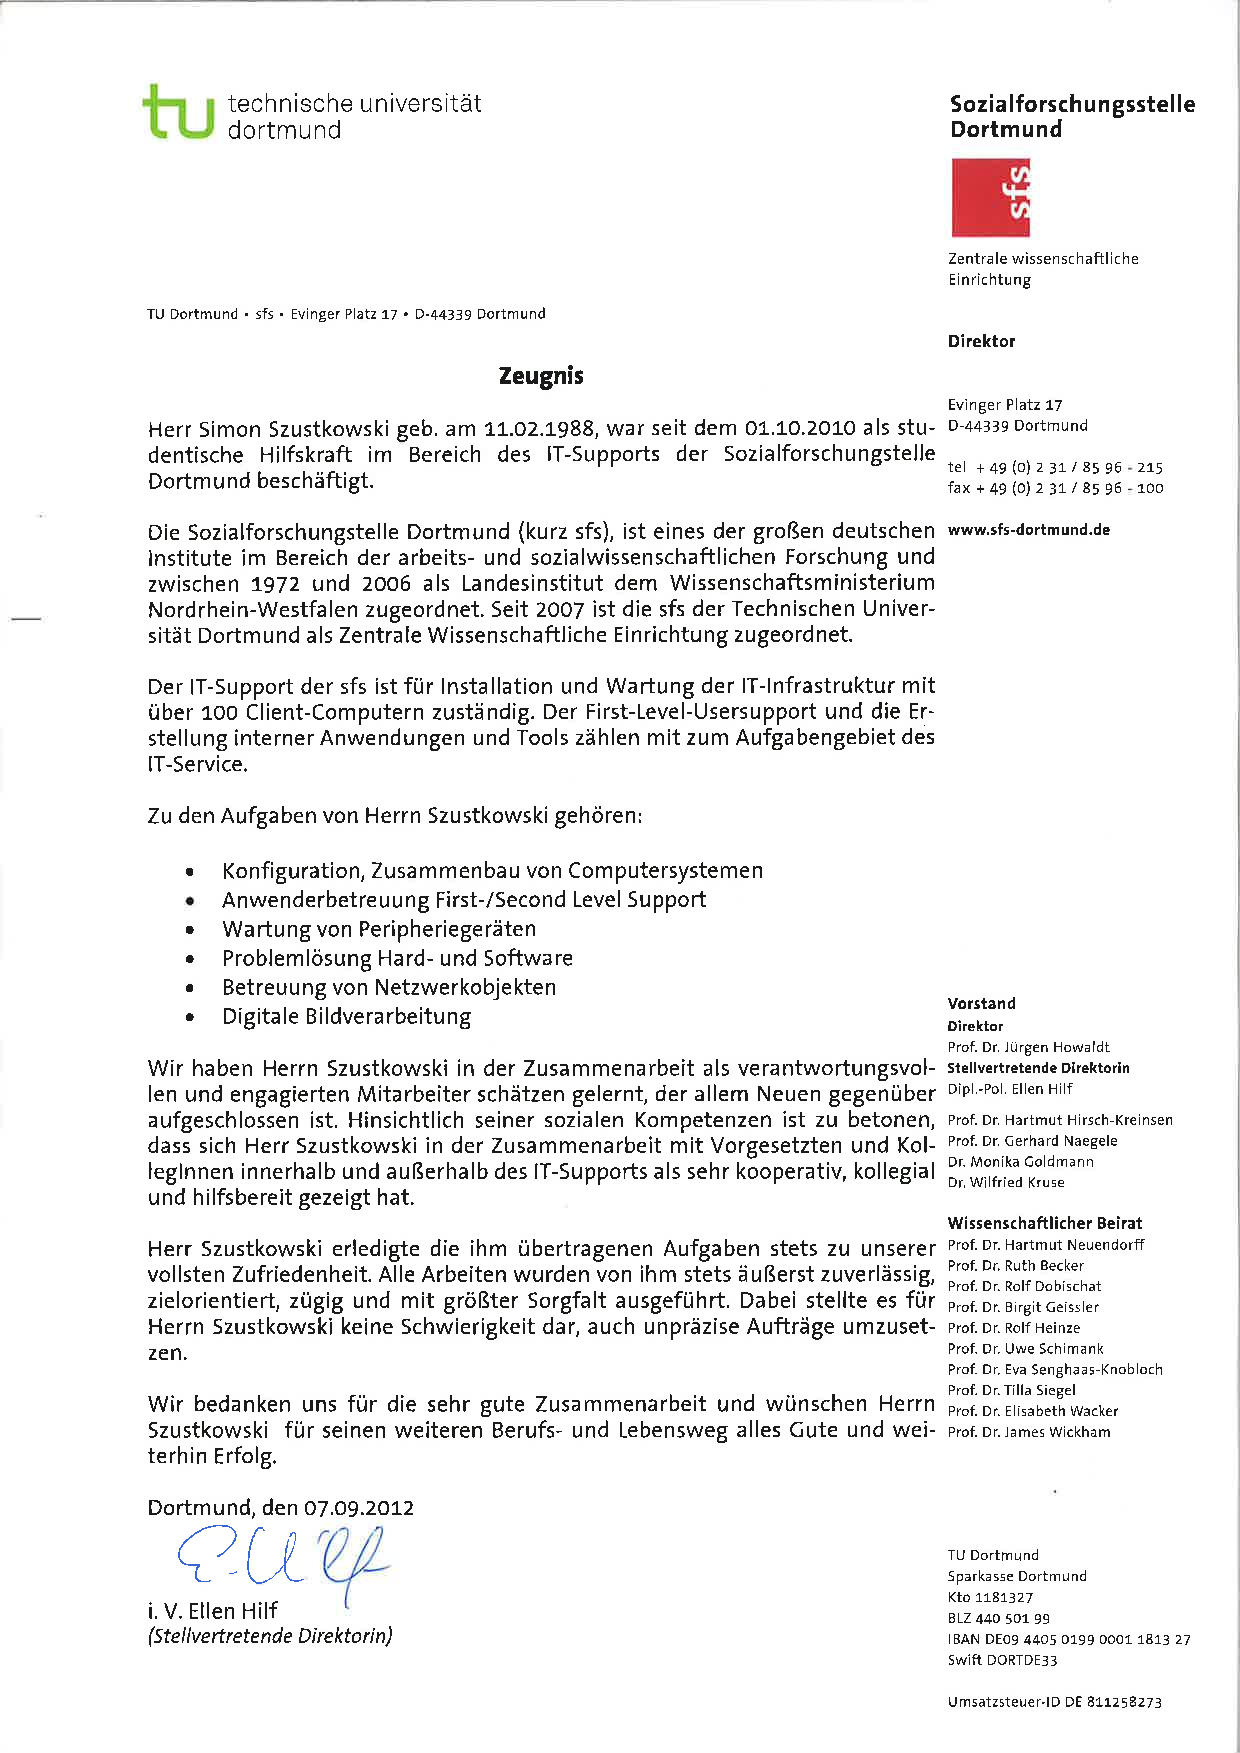
\includepdf[pages=1-]{azsfs.pdf}
%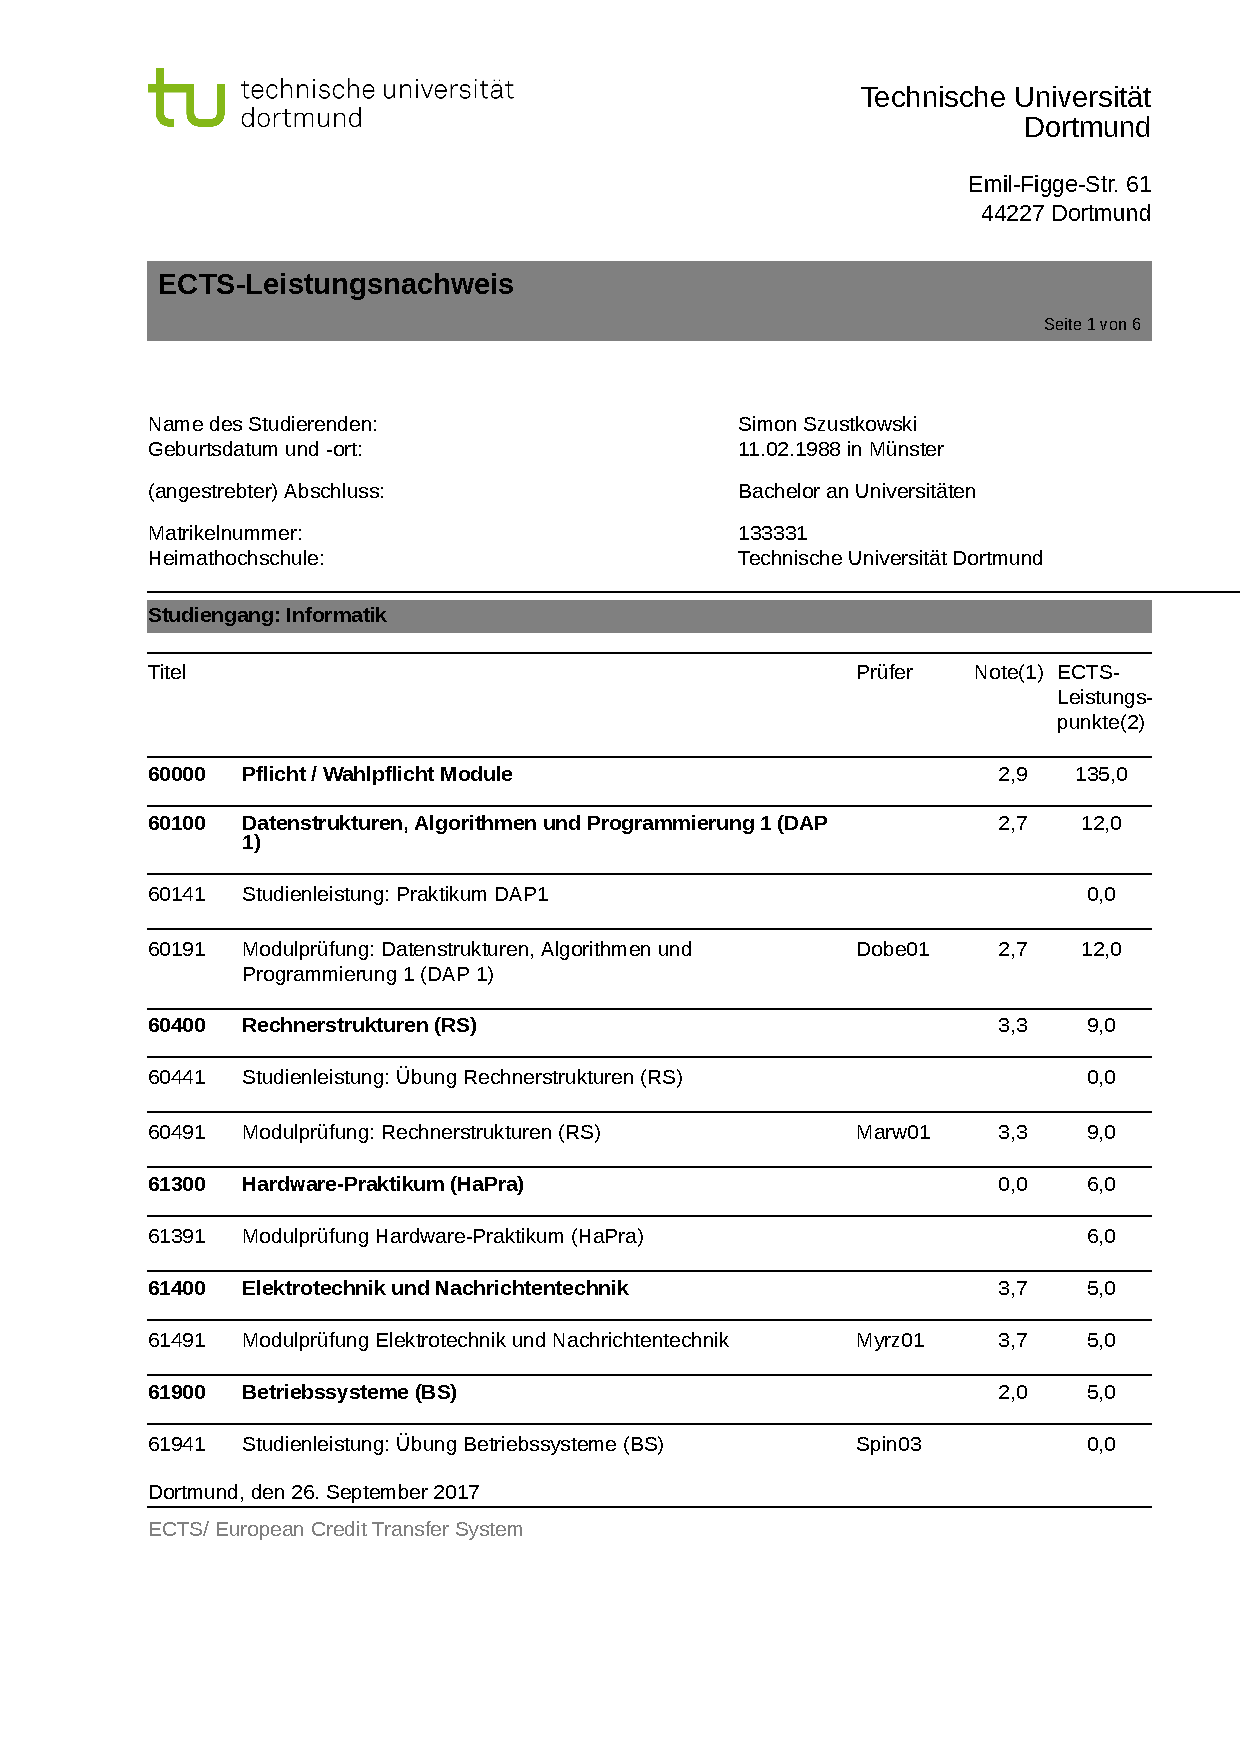
\includepdf[pages=1-]{notenspiegel.pdf}






%\chapter{Bachelor}{zeugnis}
%\vspace*{1cm}
%\begin{center}
	% \fbox{\includegraphics[height=0.85\textheight]{Bakk-Zeugnis}}	
%\end{center}

%\newpage
%\chapter{Master}{zeugnis}
%\vspace*{1cm}
%\begin{center}
	% \fbox{\includegraphics[height=0.85\textheight]{Masterzeugnis}}	
%\end{center}

%\vspace*{1cm}
%\begin{center}
	% \fbox{\includegraphics[height=0.85\textheight]{Masterzeugnis-2}}	
%\end{center}

% \newpage
% \chapter{Abschluss}{zeugnis}
% \vspace*{1cm}
% \begin{center}
% 	% \fbox{\includegraphics[height=0.85\textheight]{Abschlusszeugnis}}	
% \end{center}

\end{document}

% end of file `cv_german.tex'